\documentclass[11pt, a4paper]{report}
\usepackage{graphicx}
\usepackage[table,xcdraw]{xcolor}
\usepackage{geometry}
\usepackage[backend=biber]{biblatex}
\usepackage{float}
\usepackage{authblk}
\usepackage{anyfontsize}
\usepackage[document]{ragged2e}
\usepackage{titlesec}
\usepackage[parfill]{parskip}
\usepackage{amsmath}
\titleformat{\chapter}[hang] 
{\normalfont\huge\bfseries}{\chaptertitlename\ \thechapter:}{1em}{} 
\geometry{left=2.5cm,right=2.5cm,top=2.5cm,bottom=2.5cm}
\graphicspath{ {./images/} }

\addbibresource{bibfolder/ref.bib}

% CHECK https://www.youtube.com/watch?v=ZYvS52511oQ FOR INFO ON SETTINGS FOR biblatex

\begin{document}

\pagestyle{empty}
\centering
\fontsize{2cm}{2cm}\selectfont{Research document} \\
\vspace{2mm}
\fontsize{1cm}{1cm}\selectfont Audio digital signal processor \\
\vspace{2mm}
\large BeCreative Minor\\
\normalsize
\vspace{4cm}
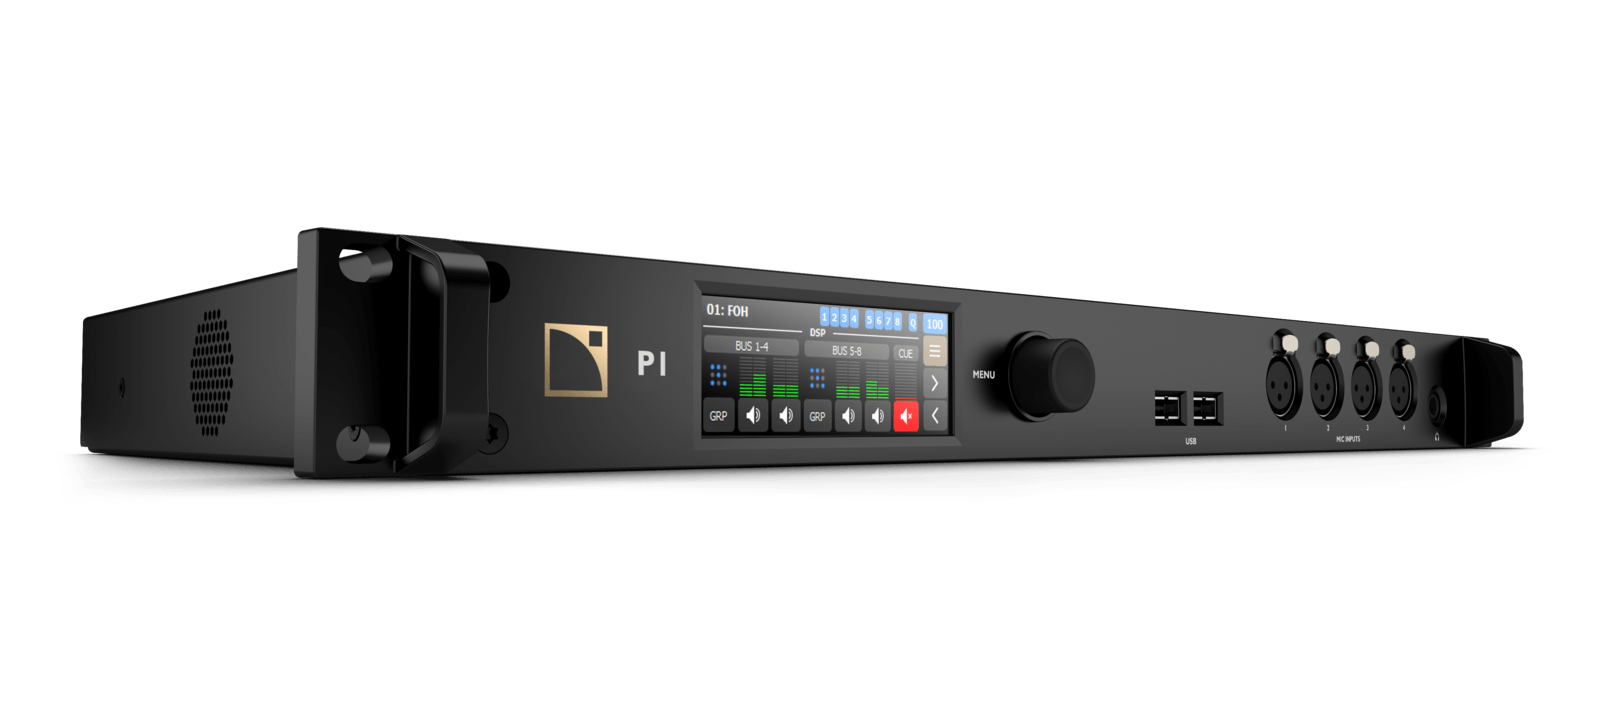
\includegraphics[width=\linewidth]{3DR_P1_Perspective.png}\\
\vfill
\normalsize Busse Lommers \\
Robin van den Dungen \\
Mahmud Gürler \\
Silas Kamphuis \\
Hein Verhallen \\
Youri Tils \\
Ahmed Abdelrahim \\
Fontys Hogescholen, De Rondom 1, 5612 AP Eindhoven \\
\today

\begin{justify}

\newpage
\tableofcontents
\thispagestyle{empty}

\listoffigures
\thispagestyle{empty}

\listoftables
\thispagestyle{empty}

\newpage
\pagestyle{plain}
\setcounter{page}{1}

\chapter*{List of Abbreviations}
\begin{table}[!h]
	\centering
\begin{tabular}{|c|c|}
	\hline
\textbf{Abbreviation} & \textbf{Explanation}        			\\ \hline
DSP                   & Digital Signal Processor    			\\ \hline
ADC                   & Analog-to-Digital Converter				\\ \hline
DAC                   & Digital-to-Analog Converter				\\ \hline
SNR 				  & Signal-to-Noise Ration    				\\ \hline
THD 				  & Total Harmonic Distortion 				\\ \hline
ENOB 				  & Effective Number Of Bits 		   		\\ \hline
SINAD 				  & Signal-to-noise and distortion ratio	\\ \hline
\end{tabular}
\caption{List of commonly used Abbreviations}
\label{Abbreviation list}
\end{table}

\chapter{Introduction}
%	\input{introduction.tex}

\chapter{Research questions}

	\chapter{Research questions}

\section{What is the best method for creating digital filters?}
    \subsection{Different mathematical methods for digital filter design}
    There are a lot of different mathematical methods for designing digital filters. Here is a large list of a lot of different methods generated by ChatGPT

    \begin{itemize}
        \setlength\itemsep{-0.3em}
        \item Fourier analysis: This method is used to decompose a signal into its frequency components. By analyzing the frequency components of a signal, it is possible to design digital filters that can remove unwanted frequency components.
        \item Z-transform: This method is used to convert the difference equation of a digital filter into a transfer function in the Z-domain. This transfer function can then be used to analyze the frequency response of the filter and to design the filter.
        \item Windowing: Windowing is a method used to design finite-duration impulse response (FIR) filters. This involves multiplying a rectangular window function with the impulse response of the desired filter to obtain a truncated impulse response.
        \item Parks-McClellan algorithm: This is a method used to design optimal FIR filters. The algorithm seeks to minimize the difference between the desired frequency response and the actual frequency response of the filter.
        \item Chebyshev approximation: This is a method used to design digital filters with a ripple in the passband or stopband. Chebyshev filters can be designed using the Chebyshev approximation method, which is based on Chebyshev polynomials.
        \item Sure, here are some more examples of mathematical methods that can be used in digital filter design:
        \item Frequency sampling: This method is used to design finite impulse response (FIR) filters. It involves specifying the desired frequency response of the filter at a set of discrete frequencies, and then using the inverse discrete Fourier transform to obtain the filter coefficients.
        \item State-space methods: State-space methods can be used to represent digital filters in a form that is amenable to analysis and design. The state-space representation consists of a set of first-order differential equations that describe the behavior of the filter over time.
        \item Bilinear transform: The bilinear transform is a method for mapping analog filters to digital filters. This involves substituting the variable s with a function of the sampling frequency and applying the inverse Laplace transform to obtain the digital filter transfer function.
        \item Impulse invariance: Impulse invariance is another method for mapping analog filters to digital filters. This involves sampling the impulse response of an analog filter and using it to obtain the impulse response of a corresponding digital filter.
        \item Pole-zero placement: This method involves placing the poles and zeros of a digital filter in specific locations to achieve a desired frequency response. This method can be used for both infinite impulse response (IIR) and FIR filters.
        \item Optimization methods: Optimization methods can be used to design digital filters that meet certain design specifications. These methods involve formulating a cost function that measures the deviation between the desired and actual frequency response of the filter, and then using optimization algorithms to minimize the cost function.
        \item Frequency transformation: Frequency transformation is a method used to transform the frequency response of a digital filter while preserving the filter's stability. This method involves applying a mathematical function to the frequency variable of the filter transfer function.
        \item Prony's method: Prony's method is used to estimate the parameters of an IIR filter from a finite set of samples. The method involves fitting an exponential signal model to the sampled data to estimate the filter coefficients.
        \item Wavelet analysis: Wavelet analysis is a method used to analyze signals in the time-frequency domain. This method can be used to design digital filters that are well-suited for signals with non-stationary frequency content.
        \item Singular value decomposition: Singular value decomposition is a method used to analyze the frequency response of a digital filter. This method involves decomposing the filter transfer function into a set of eigenvalues and eigenvectors.
        \item Genetic algorithms: Genetic algorithms are optimization methods that are inspired by biological evolution. These algorithms can be used to design digital filters that meet certain design specifications.
        \item Kalman filtering: Kalman filtering is a method used to estimate the state of a dynamic system from a set of noisy measurements. This method can be used to design digital filters that are well-suited for systems with non-stationary noise.
        \item Multirate signal processing: Multirate signal processing involves the manipulation of signals at different sample rates. This method can be used to design digital filters that are optimized for specific processing tasks, such as decimation, interpolation, and filter banks.
        \item Complex variable methods: Complex variable methods can be used to analyze the behavior of digital filters in the complex frequency domain. This method involves extending the frequency variable to the complex plane and using complex analysis techniques to analyze the filter transfer function.
        \item Lattice structures: Lattice structures are a class of digital filter structures that can be used to implement both IIR and FIR filters. These structures can be designed using mathematical algorithms that optimize the filter coefficients.
        \item Nonlinear optimization methods: Nonlinear optimization methods can be used to design digital filters that meet specific design constraints, such as passband ripple and stopband attenuation. These methods involve formulating the filter design problem as a nonlinear optimization problem.
        \item Interpolation methods: Interpolation methods can be used to design digital filters that interpolate between sampled data points. These methods involve constructing a continuous function that passes through the sampled data points and then using the function to design a digital filter.
        \item Matrix factorization methods: Matrix factorization methods can be used to analyze the frequency response of digital filters. These methods involve decomposing the filter transfer function into a set of matrix factors that can be used to analyze the filter's stability and performance.
        \item Least squares: Least squares is a method used to estimate the coefficients of a digital filter from a set of input and output data. This method involves minimizing the sum of the squared errors between the predicted and actual output data.
        \item Recursive least squares: Recursive least squares is a method used to estimate the coefficients of a digital filter from a stream of input and output data. This method updates the filter coefficients in real-time as new data becomes available.
        \item Maximum likelihood: Maximum likelihood is a method used to estimate the parameters of a digital filter from a set of input and output data. This method involves finding the parameters that maximize the likelihood of observing the input and output data.
        \item Bayesian inference: Bayesian inference is a method used to estimate the parameters of a digital filter from a set of input and output data. This method involves computing the posterior probability distribution of the filter parameters given the input and output data.
        \item Wiener filtering: Wiener filtering is a method used to design digital filters that minimize the mean squared error between the desired output signal and the filtered input signal. This method involves computing the optimal filter coefficients using the input and output statistics.
        \item Convex optimization: Convex optimization is a method used to design digital filters that meet specific design constraints, such as passband ripple and stopband attenuation. This method involves formulating the filter design problem as a convex optimization problem.
        
    \end{itemize}

    \subsection{Filter design methods}
    There are several methods that we can use to design a digital filter, the choice depends on the factor such as the filter type, complexity, and performance requirements in digital audio, sound waveforms are represented by samples. An analogue-to-digital converter (ADC) measures, or samples, analogue signal and assigns a digital value to each sample. Humans can typically hear frequencies between 20 Hz and 20 kHz. (A Hz is a cycle per second.) To adequately represent this frequency range digitally, the ADC needs to sample the audio waveform at least twice the highest audible frequency; hence we have the common sample rates of 44.1 kHz and 48 kHz.
    \begin{itemize}
        \setlength\itemsep{-0.3em}
        \item Finite Impulse Response (FIR) filters: These filters are easy to implement and provide linear phase response, but they can be computationally expensive for long filter lengths.
        \item Infinite Impulse Response (IIR) filters: These filters are computationally efficient and can achieve sharper roll-off characteristics, but they can introduce phase distortion and instability if not designed properly.
        \item Frequency sampling method: This method involves sampling the frequency response of an ideal filter and then using inverse FFT to obtain the impulse response.  
    \end{itemize}

    \section{What is the best method for creating digital effects?}
        \begin{itemize}
            \setlength\itemsep{-0.3em}
            \item Adding effects to a DSP involves implementing digital signal processing algorithms that modify the audio signal in some way. There are many different types of effects that can be implemented, ranging from simple equalization and filtering to more complex effects like reverb, delay, distortion, and modulation.
            \begin{itemize}
                \setlength\itemsep{-0.3em}
                \item To implement these effects, we would need to design digital signal processing algorithms that operate on the audio signal in real-time. This might involve using digital filter design techniques to create frequency responses that shape the audio in a desired way or using time-domain techniques like convolution to create effects like reverb or delay.
            \end{itemize}
        \end{itemize}

        Design methods are:
        \begin{itemize}
            \setlength\itemsep{-0.3em}
            \item Delay-based effects
            \begin{itemize}
                \setlength\itemsep{-0.3em}
                \item Delay-based effects involve creating one or more delayed copies of the input signal and then modifying the delay time or feedback amount to create the desired effect. \\
                Examples of delay-based effects include reverb, echo, and chorus.
            \end{itemize}
            \item Filter-based effects
            \begin{itemize}
                \setlength\itemsep{-0.3em}
                \item Filter-based effects involve using digital filters to modify the frequency content of the input signal. \\
                Examples of filter-based effects include EQ and phaser.   
            \end{itemize}
            \item Modulation-based effects
            \begin{itemize}
                \setlength\itemsep{-0.3em}
                \item •	Modulation-based effects involve using various modulation techniques, such as amplitude modulation or frequency modulation, to alter the characteristics of the input signal. \\
                Examples of modulation-based effects include tremolo, vibrato, and ring modulation.                
            \end{itemize}
            \item Distortion-based effects
            \begin{itemize}
                \setlength\itemsep{-0.3em}
                \item Distortion-based effects involve intentionally distorting the input signal to create a specific sound or tone. \\
                Examples of distortion-based effects include overdrive, fuzz, and distortion.
            \end{itemize}
            \item Pitch-based effects
            \setlength\itemsep{-0.3em}
            \item Pitch-based effects involve altering the pitch or tuning of the input signal. \\
            Examples of pitch-based effects include pitch shifting, harmonization, and auto-tune.
        \end{itemize}

      \section{What is the most suitable anti-aliasing}  

      \subsection{Causes for aliasing}
      An alias occurs when a signal above half the sample rate is allowed into, or created within, a digital system. It's the anti-aliasing filter's job to limit the frequency range of the analogue signal prior to A-D conversion, so that the maximum frequency does not exceed half the sampling rate — the so-called Nyquist limit.
      Aliasing can occur either because the anti-alias filter in the A-D converter (or in a sample-rate converter) isn't very good, or because the system has been overloaded. The latter case is the most common source of aliasing, because overloads result in the generation of high-frequency harmonics within the digital system itself (and after the anti-aliasing filter).
      The sampling process is a form of amplitude modulation in which the input signal frequencies are added to and subtracted from the sample-rate frequency. In radio terms, the sum products are called the upper sideband and the subtracted products are called the lower sideband. In digital circles they are just referred to as the 'images'.
      These images play no part in the digital audio process — they are essentially just a side-effect of sampling — but they must be kept well above the wanted audio frequencies so that they can be removed easily without affecting the wanted audio signal. This is where all the trouble starts. The upper image isn't really a problem, but if the lower one is allowed too low, it will overlap the wanted audio band and create 'aliases' that cannot be removed.
      Let's consider what occurs if we put a 10kHz sine-wave tone into a 48kHz sampled digital system. The sampling process will generate additional signal frequencies at 58kHz (48 + 10) and 38kHz (48 - 10). Both of these images are clearly far above half the sample rate (24kHz), so can be easily removed with a low-pass filter, which is the reconstruction filter on the output of the D-A converter, leaving the wanted audio (the 10kHz tone) perfectly intact. See Figure 1, above.
      However, consider what happens if our 10kHz tone is cranked up too loud and overloads the A-D converter's quantising stage. If you clip a sine wave, you end up with something approximating a square wave, and the resulting distortion means that a chain of odd harmonics will be generated above the fundamental. So our original 10kHz sine wave has now acquired an unwanted series of strong harmonics at 30kHz, 50kHz and so on.
      Note that these harmonics were generated in the overloaded quantizer and after the input anti-aliasing filter that was put there to stop anything above half the sample rate getting into the system. By overloading the converter, we have generated 'illegal' high-frequency signals inside the system itself and, clearly, overloading the quantizer breaks the Nyquist rule of not allowing anything over half the sample rate into the system.

      \begin{figure}[h]
        \centering
        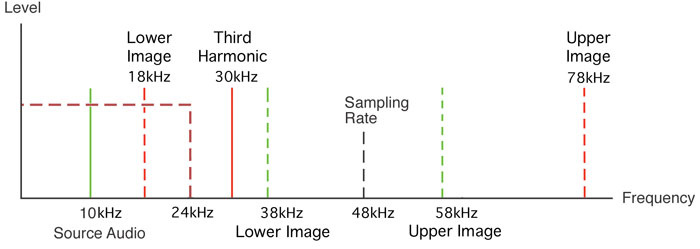
\includegraphics[width=1\textwidth]{aliasing}
        \caption{Aliasing example}
        \label{fig:aliasingexample}
    \end{figure}
    Considering just the third harmonic at 30kHz for the moment, the sampling modulation process means that this will 'mirror' around the sample rate just as before, generating additional signal frequencies at 78kHz (48 + 30) and 18kHz (48 - 30). The 18kHz product is clearly below half the sample rate, and so will be allowed through by the reconstruction filter. This is the 'alias'. We started with a 10kHz signal, and have ended up with both 10kHz and 18kHz (see Figure 2, above). Similarly, the 50kHz harmonic will produce a 2kHz frequency, resulting in another alias.
    Note that, unlike an analogue system, in which the distortion products caused by overloads always follow a normal harmonic series, in a digital system aliasing results in the harmonic series being 'folded back' on itself to produce audible signals that are no longer harmonically related to the source.
    In the simplistic example I've explained, we have ended up with aliases at 2kHz and 18kHz that have no obvious musical relationship to the 10kHz source. This is why overloading a digital system sounds so nasty in comparison to overloading an analogue system.\\
    
    \subsection{Anti-aliasing filters}
    ANTI-ALIASING FILTER THEORY
A/D Converters are usually operated with a constant sampling frequency when digitizing analog signals. By using a sampling frequency (Fs), typically called the Nyquist rate, all input signals with frequencies below fS/2 are reliably digitized.


\section{What is the optimal needed roll-off for the anti-aliasing filter for a given bandwidth such that the noise can be negligible?}
The needed roll-off of the AAF (anti-aliasing filter) depends on the bandwidth of the system, the maximum allowable noise floor of the system and the sample rate.
The maximum roll-off bandwidth can be determined by subtracting the chosen sampling frequency of the system by the two times BW of the system. As can be seen in the formula below:\\
\begin{equation} \label{eqn}
	${BW_{roll-off}=f_{s}-2BW_{system}} $
	\end{equation} 

The above formula shows that for a given BW, at a low sample rate, an AAF is needed with a very steep roll-off. If a higher sample rate is used for the same BW, an AAF with a lower roll-off is permissible. The lower the required roll-off of the AAF, the lower the order of the AAF can be. A lower order AAF will always introduce less distortion than a higher order AAF. As far as the AAF is concerned, the highest possible sample rate is desired for a given BW.\\
Using this maximum roll-off bandwidth together with the maximum allowable noise floor of the system, the minimum required roll-off of the AAF can be determined using the following formula:\\
\begin{equation} \label{eqn}
	${roll off_{min}[dB/dec] = \frac{SNR}{log_{10}(f_{s}-f_{max} / f_{max})}} $
	\end{equation} 

    \begin{equation} \label{eqn}
        ${roll off_{min}[dB/dec] = \frac{SNR}{log_{2}(f_{s}-f_{max} / f_{max})}} $
        \end{equation} 

Figure 3.2 shows a graphical representation of the AAF in the frequency spectrum of an ADC.
    \begin{figure}[h]
      \centering
     \includegraphics[width=1\textwidth]{AAF roll-off}
     \caption{Frequency spectrum of an ADC to visualize the required AAF magnitude response}
      \label{fig:AFFrolloff}
    \end{figure} \\   
    
    So according to Equation 1 by increasing the sample frequency we decrease the minimal roll-off needed for a given SNR. Therefore it would be best to choose the highest possible sample frequency.\\

        \section{What is the minimum sample frequency needed to capture the desired frequency spectrum?}
        The human hearing frequency range is 20Hz to 20kHz. According to the Nyquist theorem the sample frequency must be twice the highest measurable frequency to be able to reconstruct the original signal ${f_s>2⋅f_}$ . This would mean that the sample frequency should be at least f_s=20kHz⋅2=40kHz. \\

        \section{What is the minimum frequency range to be sampled to achieve sufficient detailed audio?}
        The best frequency response for high-quality audio devices is 20Hz to 20kHz.\\
% NEEDS REFERENCE FROM WORD STILL.

        \section{What is the lowest allowable noise for decent audio?}
            \subsection{Total Harmonic Distortion}
            Total Harmonic Distortion (THD) is the ratio between the sum of the power of all harmonics in a signal to the power of the fundamental frequency of the signal (see Equation 2 and Equation 3) \\
            \begin{equation} \label{eqn}
                ${THD(dB) = 20log \frac{\sqrt{H_{2}^{2}+H_{3}^{2}+H_{4}^{2}+...+H_{n}^{2}}} {H_{1}}}  $
                \end{equation} 

                % \begin{equation} \label{eqn}
                %     ${} $
                %     \end{equation} 

            \subsection{Aliasing intermodulation distortion}
            When signals are sampled at frequencies higher than half the sample frequency, the signal gets mirrored around half the sample frequency. This causes the mirrored signal to intermodulate with the fundamental signals and create unwanted harmonics (see Figure 2). 
            % TWO FIGURES
            The solution to prevent aliasing modulation distortion is to have the aliasing filter have full attenuation at half the sample frequency (see Figure 3). \\

            \subsection{SNR}
            Any electronic audio device (amplifier, preamp, CD player, turntable, etc.) generates more or less interference signals and background noise which are affecting the sound signal . It is the very functioning of its components (capacitors, transistors, resistors, etc.) that generates this noise.
The signal-to-noise ratio (SNR, see Figure 4) is expressed in decibels (dB) and indicates the level difference measured between the background noise generated by the circuits / components of a device (hiss when no signal passes through it) and the signal at its nominal level (defined at +4 dBu on analog devices, which corresponds to the “0” level of the VU meters of amplifiers, for example).\\
% ANOTHER FIGURE
The higher the signal-to-noise ratio of a device, the lower its background noise, in other words the more “silent” its operation. Quieter operation makes more subtle sounds more audible.
It is generally considered that a good signal to noise ratio is 60 dB or more for a phono turntable, 90 dB or more for an amplifier or CD player, 100 dB or more for a preamp.\\

% ANOTHER FIGURE
So according to this paper the total Human hearing range is 120dB. Therefore it would be best if the SNR is higher than 120dB.
Abbreviations: FS = Full Scale\\

\textbf{Idle Channel Noise}\\
Idle channel noise, in dB, is a ratio of the full scale RMS signal level to the RMS sum of all other spectral components over the specified bandwidth using a zero amplitude signal. ICN is a measure of the static noise produced by the device with a zero amplitude signal. It is useful to have good ICN performance in order to avoid an irritating noise commonly referred to as hiss, random noise, or white noise. Leakage from local sources, such as power lines, will show up and degrade ICN performance as well.\\

\textbf{Frequency Response}\\
Frequency response is the variation of the system’s output level relative to the input level across a frequency range (EQ. 3). The typical human hearing range is 20Hz to 20kHz. Therefore, audio systems with a flat response over this range seem to sound the most natural. As a performance benchmark, an in-band frequency flatness tolerance, in dB, is usually specified. For example, most conventional stereo audio systems specify a frequency flatness tolerance of ±3dB. In addition, the -3db points of the system at high and low frequency extremes are also specified. The -3dB point corresponds to the frequency at which the signal power has been reduced to one half of the normal 0dB signal level. A typical system frequency response plot is pictured in figure 1 with the -3dB points at 20Hz and 20kHz. It has been shown that human perception is capable of detecting signal amplitude differences as low as 0.1dB. However, under dynamic signal conditions, 1dB is more realistic. Table 2 lists some common frequency response examples. The frequency response of a system is usually measured with an input signal that is -20dB below full scale.\\
%Another figure and another formula

\textbf{Decibels}\\
Why Decibels? The decibel is a logarithmic unit which is used in a number of scientific discipline to compare some quantity with some reference value. Usually the reference value is the largest or smallest likely value of the quantity. We use decibels for several reasons. Quantities of interest often exhibit such huge ranges of variation that a dB scale is more convenient than a linear scale. For example, the listening level of your home stereo can vary by seven orders of magnitude. In addition, the human ear interprets loudness on a scale much closer to a logarithmic scale than a linear scale. The ‘bel’, named after Alexander Graham Bell, is the logarithmic ratio of two powers, P1 and P2, and is expressed in Equation 4.\\
%Formula
The reference power is usually based on some very small natural occurrence. An example of which is sound pressure level. The reference sound pressure level in air is 0.0002 Pa(RMS). A typical loudspeaker, with 1 watt of power at 1kHz, produces 9B of sound pressure measured at a standard distance of 1 meter. The same loudspeaker is most likely limited to about 11B of pressure. Average listening levels are usually around 6B. This makes the measurement range only 5B. Due to the small size of the bel, the more convenient decibel has become standard and is expressed in Equation 5. \\
%Formula
The decibel is often used to express the relative amplitude or power of a signal. Since power is the square of amplitude, a simple translation from Amplitude to Power can be made as in Equation 6. Some common variations on the decibel are listed below.\\
%formula
“dB FS” stands for “dB relative to full scale” and is generally used in all audio measurements unless otherwise specified. “dBr” stands for “dB relative to some absolute level.” When the absolute level is set to full scale, “dBr” is equivalent to “dB FS.” “dBV” stands for “dB relative to 1V.”\\

\subsection{Conclusion}
So for generic amplifiers such as CD player a typical SNR is 90dB. The total human ear range is 120dB. Therefore the SNR of HiFi audio system is also 120dB. Thus for a decent audio system a SNR of 90dB or higher is already sufficient. But to deliver a very good quality High-end product the SNR should be 120dB. 
But with higher bit resolution of the ADC certain signal-to-noise ratios can be neglectable. This is because with a certain amount of ADC resolution the steps are bigger than the actual noise. For example at 24 bit and 1V reference you have a resolution of approximately 60nV. This is very small, therefore allowing a lot of noise to be measured as well. Thus to attenuate the noise enough for this resolution you would need a SNR of at least: SNR=20 log⁡〖1V/60nV〗≈144dB. The typical SNR for common ADC resolutions are also shown in paragraph 1.8. 
As the SNR needs to be extremely high, which is extremely difficult to achieve, you probably just go with an SNR of 120dB. This causes a lot of noise to be measured with the 24 bit resolution. Which actually means that you can’t use all the 24 bits due to the noise. The bits that can be used are described as Effective Number Of Bits (ENOB). The equation for this term is seen in Equation 4.\\
%2 more formulas
SINAD stands for Signal-to-Noise And Distortion ratio. It is the ratio between the power of the whole signal and the noise and the distortion of the signal (see Equation 6). \\
% Formula
Note that Equation 4 assumes a full-scale input signal. Therefore when the signal level is not full-scale the ENOB calculation needs correction. \\
%Formula
So for example, with a SNR of 100dB we get an ENOB=(100dB-1.76)/6.02=16.32 bits. Thus with this attenuation of 100dB it would be useless to have 24 bits as we would never use more than 16.32 bits. A resolution of 16 bits would be the best choice as you then use every bit.
With a SNR of 120dB we get an ENOB=(120dB-1.76)/6.02=19.64 bits. This means that with a resolution of 24 bits we can’t use 4.36 bits. 
So to effectively use a 24 bit resolution we would at least need a SNR of 120dB to make a difference in resolution compared to a 16 bit resolution.\\
%figure

\section{What ADC resolution is needed such that the quantization error and noise level are on par?}
\textit{Maximum quantization error=(V_H-V_L)/(2⋅2^n )}
\textit{Where n is the number of bits.}\\

Quantization error is the difference between the analog signal and the closest available digital value at each sampling instant from the A/D converter. Quantization error also introduces noise, called quantization noise, to the sample signal. The higher the resolution of the A/D converter, the lower the quantization error and the smaller the quantization noise. The relationship between resolution (in bits) and quantization noise for an ideal A/D converter can be expressed as:\\
\begin{equation} \label{eqn}
	\text{Signal to Noise} = {-20 log(1/2^{n})} 
	\end{equation}   

%Where n is the resolution of the A/D converter in bits. S/N is the signal to noise and is expressed in dB. This relationship can also be approximated as Signal to Noise=6⋅n. Typical S/N ratios for ideal A/D converters are 144dB for 24 bits, 96dB for 16 bits, 72dB for 12 bits, and 48dB for 8 bits.\\
Where n is the resolution of the A/D converter in bits. S/N is the signal to noise and is expressed in dB. This relationship can also be approxiamted as Signal to Noise = {6n} . 
Typical S/N ratios for ideal A/D converters are 144dB for 24 bits, 96dB for 16 bits, 72dB for 12 bits, and 48dB for 8 bits.\\


\section{What ADC and DAC architexture is most suitable for this application?}
        \subsection{ADC}
        An Analog to Digital Converter (ADC) is a system that can convert analog signals into digital signals. In the case of this project: analog audio signals.
Continuous-time and amplitude analog signals are converted to discrete-time and amplitude digital signals. During this project data is lost, and noise gets added. The signal-to-noise ration (SNR) is determined by the accuracy of the ADC. This accuracy depends on the matching of the quantization levels and the true analog signal. Another factor that characterizes an ADC is the bandwidth. If the bandwidth of the ADC is twice the bandwidth of the analog signal, perfect representation of the signal is possible. 
To make the signal not cut off on low levers an ADC can implement dither. This will add a small amount of noise so that there will be more information stored than before. 
The sampling rate of the ADC is also important. The sample rate is the rate of which a continuous time signal is sampled. As mentioned before, if the sample rate is more than twice the amount of the highest frequency, perfect reproduction is possible. \\

\textbf{Types of ADCs}\\
        \textit{Direct conversion (flash)} - A direct conversion ADC uses multiple comparators that all have a certain voltage range that the comparator works in. Each comparator compares the input voltage to a reference voltage and converts it to a digital signal using a bit encoder. 
        This ADC architecture had poor energy dissipation and uses a lot of comparators to accomplish a wide range of signal.\\

        \textit{Successive approximation} - A Successive approximation ADC uses a binary search algorithm that finds the input voltage and compares it with an internal DAC (see info DAC) to converse the analog signal to a digital signal. This type of ADC is slower because this architecture of conversion tests all the weights of the algorithm and only one conversion is processed during n comparison cycles. \\

        \textit{Ramp compare} - This ADC generates a sawtooth signal that ramps up (or down) and quickly goes back to the original state. While doing this, the ADC compares the value of the ramping signal to the input signal. During this process a timer runs and stops when the signal of the input matches the ramp signal. The number of pulses the counter gave is the digital representation of the analog signal.\\

        \textit{Wilkinson} - The Wilkinson ADC charges a capacitor till it reaches the input voltage. The time it takes to discharge the capacitor is the digital representation of the amplitude of the input signal. \\

        \textit{Integrating} - With an Integrating ADC, the input voltage is ran through a integrator and can run up for a certain time. A known reference voltage than is ran through the integrator with reversed polarity. The input voltage is then functioned with the reference voltage, run-up time and run-down time. The time of the run-up and run-down is the digital output. 
        With this ADC, the resolution gets better the longer the ADC can run up. So, the ADC gets slower if the application is more demanding. \\

        \textit{Delta encoded} - The input voltage and an up-down counter DAC go through a comparator that controls the counter from the DAC. The counter changes until the DAC signal and input signal are the same. The counter is in this case the digital output.
        Delta converters have a wide range and high resolution. Although, it depends on how the input signal behaves.\\
        
        \textit{Pipelined} - A pipelined ADC has several stages. A sample and hold stage, an ADC (e.g., a flash ADC) and a DAC stage. The input signal is sampled and hold for a certain amount of time. It is then converted to a digital signal where the most significant bits are then converted back by the DAC. This process can repeat several times if necessary. For example, a 4-stage, 16-bit ADC only needs 60 comparators. 
        These ADCs are very fast, have a high resolution and can be implemented efficiently. \\
        
        \textit{Delta-sigma} - This architecture uses a feedback loop together with an analog filter. This ADC architecture has potential for high resolution, high accuracy, and low noise. This architecture works by oversampling the analog input signal and using the feedback loop to make a high-speed digital bitstream. Delta-sigma ADCs are used in high-end audio equipment. \\

        \textit{Time-interleaved} - A time-interleaved ADC exists of multiple parallel ADCs that sample every x cycles. This ADC architecture exists to correct time interleaving mismatch errors.\\

        \textit{Intermediate FM} - An ADC with an intermediate FM stage uses a voltage-to-frequency converter to convert the analog input signal into an oscillating frequency. Then a frequency counter is used to read this frequency and output a digital signal.\\

        \textit{Time-stretch} - This ADC can digitize a wide bandwidth analog signal that can normally not be converted by a conventional ADC. A time-stretch ADC slows down the input signal and compresses the bandwidth. A normal ADC can now capture this slowed-down signal.\\
        
        The ADCs that are used the most in audio applications are: Sigma-delta, Successive approximation and pipelined.\\

        \subsection{DAC}
        A Digital-to-Analog converter converts digital signal into analog signal. Architectures of different DACs is also determined by factors like resolution and sampling frequency. DAC’s can make a signal worse so choosing the right architecture is important for this project. So in essential, a DAC does the reverse thing an ADC does.
An audio DAC is a low frequency, high resolution type DAC. Higher resolutions means more levels of an analog signal can be reached, thus a better audio quality. \\

        \textbf{Types of DACs}\\
        There are a couple of types of DACs frequently used in the audio world. Each has different focusses. Some DACs have the focus on the least significant bit, and others have the focus on the most significant bit. Sometimes, more than one type of architecture is used to help fix certain properties. Segmented DACs are DACs that are designed out of different architectures for specific performances. 

        \textit{The binary weighted} - The binary weighted DAC has several bit inputs that lead into an operational amplifier where all the inputs have a powers-of-two weighting with the current voltage. This conversion method is very fast but has poor accuracy. Another disadvantage is that the power dissipation of a binary weighed DAC is very high. \\

        \textit{The R2-R ladder(or binary ladder)} - The R2-R ladder DAC only uses two values of resistors (which makes accuracy better and fabrication easier) and is easily scalable. Because of this, de DAC does work slower than the binary weighted DAC. With this type of DAC there is some delay due to switching based on the inputs.\\

        \textit{Delta-sigma} - In the ADC section there was a sigma-delta ADC. The delta-sigma DAC is the exact opposite. It uses an interpolation filter to increase the sample rate and to reduce the time, so that the sample frequency is increased by four times. Then the signal goes through a modulator which acts as a High-Pass Filter for the quantization noise and as a Low-Pass Filter to the signal. After this process the high-speed bit-stream is converted to analog by a 1-bit DAC. The signal is converted serially.
        This DAC is one the fastest and most precise DAC.\\

        \textit{Pulse-Width Modulation(PWM)} - The PWM DAC uses a fixed frequency signal to create a series of pulses with the width proportional to the amplitude of the digital signal. This is a relatively simple DAC that is very accurate.\\

        There are also oversampling DACs. This DACs take the original signal and oversamples it to a higher frequency. After this step the signal is filtered to remove noise. These DACs can achieve a higher precision and quality signal. \\

        \textbf{Segmented DAC}\\
        As said before, to fulfill certain specifications, multiple DACs are joined together as a segmented DAC. For example: A thermometer-coding DAC is used for the most significant bit, and a binary-weighted DAC is applied for the least significant bit. \\

        \textbf{Best DAC and ADC architectures for audio use}\\
        \noindent For this project, ADC- and DAC architectures should be chosen for audio signals. The projects aim is to have high quality audio processed so the ADCs and DACs should be capable of converting high quality signals into converted high quality signals. The minimum required sample rate is 44.1 kHz. But higher sample rates such as 96 and 192 kHz are favored. The ADCs and DACs of choice should be at least 16 bits, but 24 bits is preferred. The SNR depends on how many bits the ADC and/or DAC has. For a 24 bits component de SNR should be close to 144dB and for 16 bits close to 96dB. 
There are a couple of brands that make audio ADCs and DACs. Texas Instruments and Asahi Kasei Microdevices are two big sellers of ADC and DAC chips. Because of the data available, and the widely available chips that they offer, Texas Instruments is the preferred company for this project.
Texas Instruments offers a wide spectrum of ADCs and DACs with the price ranging from a few euros to several hundred euros.
For this project with these specific requirements (and depending on stock) there can be made a list of good choises.\\

\underline{ADC}\\
TI PCM18xx Series (24 bit, low power, 96-192kHz)
This ADC series has a lot of different models but are all ranging from 96 to 192kHz. The PCM18xx’s are Delta-Sigma converters and are designed for audio processing application such as amplifiers, receivers, and audio recorders. The 1800 series is inexpensive (around 3 to 8 euros.) \\

\underline{DAC}\\
TI PCM17xx Series (24 bit, 96-192kHz)
The TI PCM17xx series is a 24 bits DAC and is comparable with the 18xx series from the ADC. It’s fast, precise, and inexpensive. These DAC chips are also built on the Delta-Sigma architecture. Cost of a chip is around 3 to 10 euros. 

The 16 bits DACs and ADC cost the same as the 24 bits but are noticeably slower and have a lower SNR.\\

\section{What kind of processor is most suitable for this application?}
For DSP applications most of the time an FPGA or dedicated DSP is used. They both are great and will work for our application. 
An DSP is mostly used in market segments that have a very specific use case. The specifications for these applications are very clear and will stay the same for the whole development process. This is because the hardware architecture is inflexible. This makes them unsuitable for dynamic applications. General-purpose DSPs cost between 1- and 300-euro dependent on their features and applications. In general, an DSP is easy to implement, and use. Most DSPs use C code and are well documented. 
FPGAs are designed with logic elements and memory that are configurable. Therefore, an FPGA can be used for a wild range of applications of which digital signal processing. This also means that an FPGA is more modular so the end user can implement multiple hardware designs to ensure the FPGA fits in to specific requirements. FPGAs are equipped with embedded memory, embedded processors such as ARM Cortex and DSP blocks. The DSP blocks are there to perform specific DSP tasks that the normal logic elements cannot handle efficiently. In general FPGAs are more expensive around 100 to 1000 euro. There are less expensive FPGAs but there are generally not used for DSP applications.\\

\section{What is the permittable jitter for accurate audio?}

\section{What is the maximum allowable ripple on the reference voltage for the ADC and DAC?}
        \subsection{ENOB (Effective Number of Bits)}
        Analog-to-Digital Converter (ADC) resolution can be used to describe the general performance of an ADC. Resolution and accuracy are terms that are often interchanged.
The resolution of an A/D converter (ADC) is specified in bits and determines how many distinct output codes (2n) the converter can produce. In other words, a resolution is the smallest voltage increment corresponding to a 1 LSB change. It's an important ADC specification because it determines the smallest analog input signal an ADC can resolve.
For example, an 8-bit ADC produces 28 or 256 output codes. The accuracy of the ADC determines how close the actual digital output is to the theoretically expected digital output for any given analog input. In other words, the accuracy of the converter determines how many bits in the digital output code represent useful information about the input signal. The accuracy of the ADC is a function of its internal circuitry and noise from external sources connected to the ADC input. In some cases, extra bits of resolution that are beyond the accuracy of the ADC can be beneficial.\\

        \subsection{ADC Effective Resolutions}
        Effective resolution describes the useful bits from an Analog to Digital conversion with respect to the input noise. Effective Number of Bits (ENOB) is often used to specify ADC effective resolution. ENOB is not the same as the actual resolution of the ADC. Effective resolution is expressed using two units of measure, the specification of bits rms (0.707) refers to the output data. Effective resolution predicts the probability of a conversion level of repeatability of 70.7% for an input signal.
1.12.2.1	Calculation
ENOB equation (based on an ideal ADC’s Signal-to-Noise Ratio (SNR): SNR = (6.02) (ENOB) + 1.76 dB where N is the ADC’s resolution. ENOB = (SNR - 1.76)/6.02.

        \subsection{Delta-Sigma A/D Converters Resolution}
        Delta-Sigma ADCs can provide resolutions as high as 24 bits. A given 24-bit Delta-Sigma converter may only provide 16 bits of accuracy. In this case, the 8 LSB’s represent random noise produced in the converter. However, these noise bits are used with digital filter algorithms to increase the useful measurement resolution at the expense of a lower sampling bandwidth.\\
%FORMULA
        \textbf{Effective Number of Bits (ENOB) of a Delta-sigma ADC is a function of the ADC's resolution in bits and its standard deviation:}
      %FORMULA
      
      \subsection{Over Sampling Ratio (OSR)}
      Both from plausibility arguments in the time domain, and from explicit calculation in the frequency domain, it appears that the modulator circuit holds the key to the sigma–delta ADC’s performance; that is, its ability to quantize an
analog input signal with a resolution considerably greater than the oversampling ratio. Furthermore, that figure of merit (Neff/log2OSR, where Neff is the effective number of bits in the quantized digital output) grows with modulator complexity: contemporary ADCs employ “higher-order” modulators, meaning that the single difference amplifier and integrator is replaced with several cascaded stages of difference amplifier plus integrator, each driven from the common bitstream (see Figure 13.55).81 Higher-order modulators are widely used, because they extend the dynamic range without having to increase the oversampling ratio (see below); they also suppress to a large extent the idle tones (see §§13.9.9 and 13.9.10) that afflict first-order modulators. Although our time-domain musings above may be helpful (if only to make plausible the excellent dynamic ranges that are claimed), any serious analysis must use.
the frequency-domain approach. The latter shows that a higher-order modulator (constructed with m integrators) modifies the noise shaping such that the in-band quantization noise (i.e., dc to fmax) is suppressed as OSRm+0.5, where m is the modulator order (m=1 for Figure 13.51). Put another way, each doubling of the oversampling ratio suppresses quantization noise so as to increase the dynamic range by m + 12 bits; or, to state it in terms of modulator order, the effective number of bits (ENOB) is the log2 of the oversampling ratio (e.g., 6 for OSR=64) multiplied by m+ 12 (thus, for example, ENOB≈15 for a second-order modulator with oversampling ratio of 64). The graph in Figure 13.56 shows the theoretical maximum dynamic range of a delta–sigma ADC as a function of oversampling ratio and modulator order.82 Another technique for extending dynamic range, speed or both, is to design a modulator that generates a modulated “wordstream” that is more than one bit wide. In Figure 13.51, for example, the 1-bit ADC, 1-bit DAC, and 1-bit register would be replaced with analogous 2-bit (4-level) components. There are lots of clever tricks to address imperfections in the multibit converters within the modulator (for example, cyclically exchanging bit positions to average out nonlinearities caused by offsets); they are well beyond the scope of this book.
Delta–sigma converters are adored by the professional audio community, owing to their combination of resolution, inherent anti-aliasing, noise shaping, and monotonicity. (See Table 13.10.) If you open up pretty much anyone’s high-quality audio gear, you’ll probably find a circuit based around a 24-bit, 192 ksps 128× oversampling delta–sigma ADC; and chances are it will be a part from Cirrus (e.g., the CS5381) or AKM (e.g., the AK5394A). These parts seem to have “long legs” – they have been around for many years and represent good value in terms of price and performance Audio ADCs universally use delta–sigma technology, but they differ greatly from their industrial ADC counterparts in the delta–sigma table. They generally have poor gain accuracy (5\% to 10\%) and dc offset (∼25 mV), inpart because these don’t matter in the audio field. On the other hand, they do offer 0.1 dB or 1\% stereo-channel gain matching. They’re usually wired with ac-coupling, and they also have an internal digital highpass filter (typically ∼1 Hz).96 They are meant to operate at specific audio data rates, and they employ specialized audio PCM data output interfaces (I2S, TDM, etc.). Compared with industrial ADCs they have high latencies (data-output delays) of 12 to 63 sample intervals, even though they may advertise “low latency” (by which they mean small compared with, say, one millisecond of time delay). They have unique audio specifications, like A-weighted SNR, and spectral analysis-derived THD+N distortion specs.Figure 13.68 Shows a straightforward signal conditioning circuit, adapted from AKM’s evaluation board, not unlike the innards of many commercial audio digitizers. The 5534 op-amp seems to be the perennial. favorite (it’s been around for at least three decades), inexpensive and “good enough.” Although you can do better interms of distortion, what seems to matter most to audiophiles is dynamic range (set by the ADC resolution and the noise level); harmonic distortion at 0.001\% is inaudible. However, we prefer full differential signal-conditioning circuits for high-performance audio ADCs, as described expansively in Chapter 5 (see Figures 5.70 and 5.102).97 See §5.14.2E for more about pro-audio signal levels.\\

        \subsection{Usecase of the CS5523-BS (example)}
        %FIGURES 2
        LDO output is 1µV p-p, this means even before the ADC the reference voltage will have a very low ripple on the output. The CS5381 ADC itself has a typical PSRR of 65dB. \\
\subsubsection{Calculation}
As calculated before the LSB for a 24-bit ADC with a 3V reference voltage is 178nV (see header 1.12.2.1 Calculation). Therefore, the reference voltage must be below the LSB voltage. The combination of the LDO ADR440 and the CS5381 ADC this is possible.\\
%FORMULA

        \section{How much RAM does the system need?}
        The product should be able to store some data. This is needed for some of the audio effect we want to make. The size of the data is dependant of the sample rate, amount of bits and time u want to safe. The following formula can be used to calculate the size:
Filesize=(sampling frequency*bit depth*length)/8  \\
The answer of this formula will be the file size in bytes. If we want to make an high quality audio DSP we probably need to use a sampling frequency of 192KHz and a bit depth of 24bit. The time is dependant on the amount of delay we want to add. Lets say for now we want to be able to store 6 seconds of audio data.
Filesize=(192.000*24*6)/8=3456000=3.456 MB\\
This is the amount needed to store 6 seconds of mono audio.
If we want to have 6 channels of audio each able to store 6 sec of data the total needed RAM will be. 
3.456 MB*6=20.736MB\\

        \section{How much flash does the system need?}
        Depends on the program size.

        \section{What power supply topology is best suited for each part of the sytem?}
        The most suitable power supply topology depends on the application. For example, switch mode power supplies have the advantage that they can achieve a high efficiency and therefore generally dissipate less power than linear voltage regulators. I say generally because for applications requiring very little power, linear voltage regulators can still be more efficient because they have lower idle losses than switch mode power supplies.
Furthermore, switch mode power supplies produce noise on the power supply lines. This noise can be significantly reduced by proper design of switch mode power supplies, but switching power supplies are still not the most suitable power supplies to use for powering noise sensitive components.
It is best to use a linear voltage regulator to power noise-sensitive components since these linear power supplies don't generate switching noise. The audio DSP will have to use a combination of switch mode power supplies and linear voltage regulators. This is to be able to use the benefits of both.
For example, a switch mode power supply will be necessary to create a negative voltage if the system is only powered by a single supply voltage (such as from a laptop charger, for example). It is not possible to convert a positive voltage into a negative voltage with linear voltage regulators. Therefore, in some cases two power supplies are used, which increases the cost of the system.
Figure 10 shows a global overview of the power supply section of an audio DSP. This is used as an reference to show where which power supply topology can best be used. As shown in Figure 10 a combination of switching voltage regulators and linear voltage regulators will be used throughout the audio DSP. The digital domain will be powered by switching regulators since this domain is not very noise sensitive. The analog domain will be powered by low noise linear voltage regulators which in some cases will be pre-regulated by switching regulators.\\
%FIGURE
Because switching regulators soon have a few millivolts of ripple voltage, it is necessary to thoroughly filter this incoming voltage because otherwise the noise of the switching regulators will end up with the noise sensitive analog section. This is because in datasheets of linear voltage regulators manufacturers often throw high PSRR (power supply rejection ratio) values, but this PSRR is actually frequency and temperature dependent. Thus, it is common for the PSRR to decrease with frequency as seen in Figure 13. Figure 14 shows a typical PSRR curve of a linear voltage regulator over temperature.\\
%TWO FIGURES
Since the linear voltage regulators as seen in Figure 12 will in all cases be powered by switching regulators which have high-frequency switching noise, it is important that the linear voltage regulators already get some pre-noise suppression. The simplest method for this is an RC filter. For a standard RC LPF, the cut-off frequency can be calculated using the formula below:\\
%FORMULA
To get a very low cutoff frequency and a high PSRR, either the resistance value R must become very large, so that the filter can no longer supply current because the output voltage would otherwise drop too far, or the capacitance C must become unreasonably large, making it very physically very large. and gets expensive. This behaviour can be easily improved by adding a transistor whose collector is connected to the (noisy) input voltage, the base is connected to the output of the RC network and the emitter forms the output. What this circuit effectively does is it multiplies the capacitance of the capacitor by the hFE of the transistor. This is because most of the current flows through the transistor and the capacitor therefore sees less ripple current. The cutoff frequency of the capacitance multiplier can therefore be calculated as follows:\\
%FORMULA
Figure 11 shows the principle of the capacitance multiplier circuit. It is important to realize that this is not a voltage regulator because the output voltage simply fluctuates with the input voltage and there is always voltage across the collector-emitter junction of the transistor.\\
%FIGURE

        \section{How is it ensured that the USB input of the processor is recognized by Windows as an audio device?}
        It is the intention that the USB input of the processor is recognized by Windows as an audio device so that it can be used for Spotify or YouTube, for example. For this, the processor must be able to sample the USB data and tell the computer what kind of device it is. A Teensy 4.0 microcontroller can be used for this, which has software libraries that make this implementation straight forward. This Teensy can transfer the USB data lossless to I2S data for the processor. The processor must be able to receive this I2S data anyway since that protocol is used for almost all audio ADCs and DACs. At the same time, the microcontroller could also be used to run the UI to send the new filter coefficients to the processor.\\
        MAX3421E\\
        MCP2221A\\
        MCP2210\\




        








% Bibliography with heading so it pops up in the table of contents (idkwhy but this is how it works)
\printbibliography[
	heading=bibintoc,
	title={Bibliography}
]

\appendix

\chapter{Appendix A}

\end{justify}
\end{document}
